\chapter{Launch and Deployment}
\definecolor{blue}{rgb}{0.2,0.5,0.8}
The rocket selected to launch the constellation is Electron, from Rocket Lab enterprise.    It is a two stage rocket capable of launching 24 3U CubeSats every week at a LEO orbit with a range of inclinations from 39.2 to 99. The cost per launch is 5.760.000 US dollars. The basic dimensions of the electron are 17 m long and 1.2 m diameter.   
\begin{figure}[H]
\begin{center}
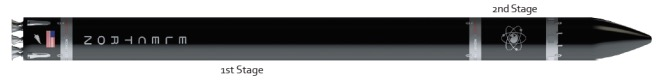
\includegraphics[scale=0.6]{Image2.jpg} 
\caption{Electron Rocket}
\end{center}
\end{figure}
\begin{figure}[H]
\begin{center}
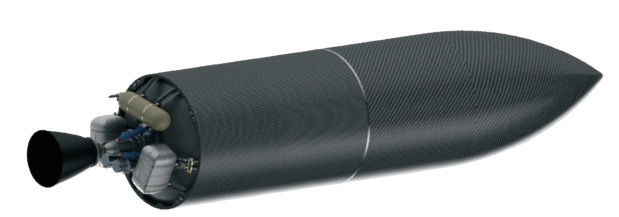
\includegraphics[scale=0.45]{secondstage.jpg} 
\caption{Electron Rocket}
\end{center}
\end{figure}
\begin{table}[H]
\begin{center}
\begin{tabular}{|c|c|c|}
\hline
\rowcolor[gray]{0.80}\textbf{Event}&\textbf{Time(s)}&\textbf{Altitude(km)}\\
\hline
Lift-off&0&0\\
\hline
Max Q&79&11\\
\hline
Stage 1 separation&152&69\\
\hline
Stage 2 ignition&159&69\\
\hline
Fairing separation&183&110\\
\hline
Stage 2 apogee kick&457&284\\
\hline
Engine cut off&3157&540\\
\hline
Payload separation&3200&542\\
\hline
\end{tabular}
\caption{Injection manouver}
\end{center}
\end{table}
The cycle of the constellation is shown in the next figure. As it can be seen, there will be a launch every week so it will take 9 weeks to put in orbit all the cubesats. After 5 years the constellation will be replaced. The replacement strategy is designed in a way that will not affect the performance of the constellation in any way. To acomplish this, when a new plane is placed the old plane will be shuted down and will decay.    
\begin{figure}[H]
\begin{center}
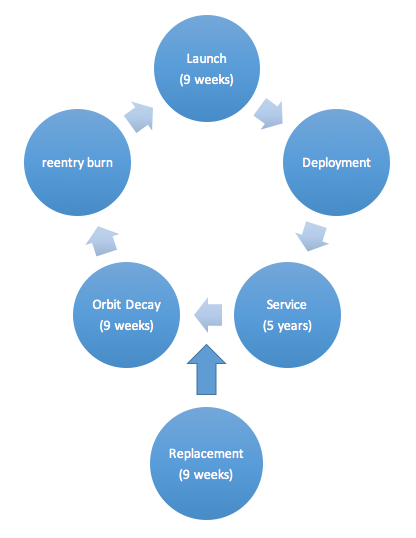
\includegraphics[scale=0.6]{Diagrama.png} 
\caption{Cycle of the Astrea Constellation}
\end{center}
\end{figure}


